\section{Results}

\subsection{Kullback-Leibler divergence(KL divergence)}
To understand the quality of the generated data, we measured the similarity of the signal by the KL divergence process.
The KL divergence was measured by comparing all pairs of train set, test set, augmented set, and train set mixed with the difference ratio of the augmented set (25\%, 50\%, 75\%, 100\%).
We randomized the augmentation data for this process 100 times and averaged the result.
Overall, our method increases similarity as the ratios of augmented data are increased.
When ratios are increased, the similarity for the SmoothTimeMask, Noise Addition, and FTSurrogate approaches that of the non-augmented data.
On the other hand, as the augmented data from frequency shift increases, the similarity declines.

% WaveGrad
\begin{table}[ht]
    \centering
    \caption[The result of KL divergence]{The result of the study of KL divergence of raw EEG dataset and data augmentation from \texttt{WaveGrad}.}
    \label{tab:KL-wavegrad}
        {\small\begin{tabular}{rccccccc}
        \br
        \multirow{2}{*}{No.} & Train vs & Train vs & Test vs & \multicolumn{4}{c}{Train with x\% of Augmentation vs Test} \\ 
        \cline{5-8} 
                             & Test     & Augment  & Augment & 25\%          & 50\%         & 75\%         & 100\%        \\
        \mr
        1                    & 2949.63  & 1582.51  & 1988.35 & 2757.15       & 2623.40      & 2525.57      & 2486.21      \\
        2                    & 1641.60  & 2970.01  & 2749.47 & 1887.98       & 2009.06      & 2118.49      & 2222.43      \\
        3                    & 2203.27  & 2800.51  & 2671.86 & 2298.26       & 2382.90      & 2416.10      & 2410.30      \\
        4                    & 2559.50  & 2193.34  & 1775.89 & 2390.33       & 2291.63      & 2240.40      & 2176.35      \\
        5                    & 2238.52  & 1870.57  & 2045.00 & 2215.49       & 2170.81      & 2146.55      & 2167.71      \\
        6                    & 1935.63  & 2069.20  & 2247.53 & 1999.40       & 2061.10      & 2067.91      & 2103.15      \\
        7                    & 2704.38  & 1808.16  & 2024.06 & 2564.74       & 2482.31      & 2424.12      & 2381.11      \\
        8                    & 3245.50  & 1398.65  & 1779.83 & 2946.14       & 2752.42      & 2628.08      & 2497.71      \\
        9                    & 2313.45  & 2123.10  & 2145.52 & 2290.44       & 2253.48      & 2231.11      & 2201.39      \\
        \mr
        Average              & 2421.27  & 2090.67  & 2158.61 & 2372.21       & 2336.35      & 2310.92      & 2294.04      \\
        \br
        \end{tabular}}
\end{table}

% noiseadd
\begin{table}[ht]
    \centering
    \caption[The result of KL divergence]{The result of the study of KL divergence of raw EEG dataset and data augmentation from \texttt{Noise Addition}.}
    \label{tab:KL-noiseadd}
        {\small\begin{tabular}{rccccccc}
        \br
        \multirow{2}{*}{No.} & Train vs & Train vs & Test vs & \multicolumn{4}{c}{Train with x\% of Augmentation vs Test} \\ 
        \cline{5-8} 
                             & Test     & Augment  & Augment & 25\%          & 50\%         & 75\%         & 100\%        \\
        \mr
        1                    & 3096.06  & 5.50     & 3136.14 & 3098.35       & 3129.45      & 3084.07      & 3082.39      \\
        2                    & 1825.54  & 8.51     & 1855.50 & 1847.41       & 1842.47      & 1840.31      & 1847.95      \\
        3                    & 1931.80  & 0.79     & 1883.10 & 1902.96       & 1899.25      & 1896.77      & 1929.07      \\
        4                    & 2236.07  & 9.64     & 2253.03 & 2214.81       & 2234.90      & 2242.26      & 2226.55      \\
        5                    & 2412.31  & 2.90     & 2417.18 & 2428.51       & 2407.26      & 2424.61      & 2411.43      \\
        6                    & 1658.42  & 5.86     & 1665.17 & 1674.19       & 1682.36      & 1661.31      & 1654.97      \\
        7                    & 2670.83  & 3.02     & 2627.48 & 2656.17       & 2653.48      & 2647.57      & 2675.15      \\
        8                    & 2492.82  & 4.33     & 2477.18 & 2486.57       & 2499.74      & 2485.40      & 2502.85      \\
        9                    & 2527.24  & 3.69     & 2534.68 & 2556.71       & 2575.44      & 2532.34      & 2514.06      \\\mr
        Average              & 2316.79  & 4.91     & 2316.61 & 2318.41       & 2324.93      & 2312.74      & 2316.05      \\
        \br
        \end{tabular}}
\end{table}

% FTSurrogate
\begin{table}[ht]
    \centering
    \caption[The result of KL divergence]{The result of the study of KL divergence of raw EEG dataset and data augmentation from \texttt{FTSurrogate}.}
    \label{tab:KL-FTSurrogate}
        {\small\begin{tabular}{rccccccc}
        \br
        \multirow{2}{*}{No.} & Train vs & Train vs & Test vs & \multicolumn{4}{c}{Train with x\% of Augmentation vs Test} \\ 
        \cline{5-8} 
                             & Test     & Augment  & Augment & 25\%          & 50\%         & 75\%         & 100\%        \\
        \mr
        1                    & 3096.06  & 1763.78  & 2161.28 & 2923.06       & 2778.94      & 2705.45      & 2639.85      \\
        2                    & 1825.54  & 2892.79  & 2890.44 & 2057.60       & 2149.51      & 2285.96      & 2365.13      \\
        3                    & 1931.80  & 2509.07  & 2393.08 & 2037.76       & 2091.94      & 2106.68      & 2157.68      \\
        4                    & 2236.07  & 1872.45  & 2087.45 & 2209.30       & 2186.28      & 2157.86      & 2162.64      \\
        5                    & 2412.31  & 1953.67  & 2062.80 & 2348.90       & 2315.24      & 2255.40      & 2231.07      \\
        6                    & 1658.42  & 2592.67  & 2411.42 & 1811.03       & 1916.95      & 1992.26      & 2062.44      \\
        7                    & 2670.83  & 1920.34  & 2195.68 & 2545.19       & 2505.66      & 2502.45      & 2440.79      \\
        8                    & 2492.82  & 2078.85  & 2220.79 & 2421.70       & 2389.56      & 2381.83      & 2342.94      \\
        9                    & 2527.24  & 2457.15  & 2208.62 & 2448.97       & 2416.09      & 2369.63      & 2353.87      \\\mr
        Average              & 2316.79  & 2226.75  & 2292.40 & 2311.50       & 2305.57      & 2306.39      & 2306.27      \\
        \br
        \end{tabular}}
\end{table}

% SmoothTimeMask
\begin{table}[ht]
    \centering
    \caption[The result of KL divergence]{The result of the study of KL divergence of raw EEG dataset and data augmentation from \texttt{SmoothTimeMask}.}
    \label{tab:KL-SmoothTimeMask}
        {\small\begin{tabular}{rccccccc}
        \br
        \multirow{2}{*}{No.} & Train vs & Train vs & Test vs & \multicolumn{4}{c}{Train with x\% of Augmentation vs Test} \\ 
        \cline{5-8} 
                             & Test     & Augment  & Augment & 25\%          & 50\%         & 75\%         & 100\%        \\
        \mr
        1                    & 3096.06  & 0.00     & 3096.07 & 3104.42       & 3093.37      & 3099.79      & 3070.69      \\
        2                    & 1825.54  & 0.00     & 1825.54 & 1821.42       & 1824.01      & 1828.32      & 1838.73      \\
        3                    & 1931.80  & 0.00     & 1931.82 & 1957.14       & 1922.34      & 1938.24      & 1938.16      \\
        4                    & 2236.07  & 0.00     & 2236.08 & 2230.66       & 2191.80      & 2251.39      & 2225.41      \\
        5                    & 2412.31  & 0.00     & 2412.31 & 2398.37       & 2426.97      & 2401.76      & 2412.11      \\
        6                    & 1658.42  & 0.00     & 1658.42 & 1651.92       & 1674.98      & 1670.55      & 1649.18      \\
        7                    & 2670.83  & 0.00     & 2670.83 & 2675.50       & 2672.44      & 2658.61      & 2673.53      \\
        8                    & 2492.82  & 0.00     & 2492.82 & 2491.67       & 2502.79      & 2544.00      & 2477.89      \\
        9                    & 2527.24  & 0.00     & 2527.24 & 2549.82       & 2571.61      & 2509.95      & 2510.61      \\\mr
        Average              & 2316.79  & 0.00     & 2316.79 & 2320.10       & 2320.04      & 2322.51      & 2310.70      \\
        \br
        \end{tabular}}
\end{table}

% Frequency shift
\begin{table}[ht]
    \centering
    \caption[The result of KL divergence]{The result of the study of KL divergence of raw EEG dataset and data augmentation from \texttt{Frequency shift}.}
    \label{tab:KL-FrequencyShift}
        {\small\begin{tabular}{rccccccc}
        \br
        \multirow{2}{*}{No.} & Train vs & Train vs & Test vs & \multicolumn{4}{c}{Train with x\% of Augmentation vs Test} \\ 
        \cline{5-8} 
                             & Test     & Augment  & Augment & 25\%          & 50\%         & 75\%         & 100\%        \\
        \mr
        1                    & 3096.06  & 7785.11  & 9331.32 & 4327.54       & 5166.36      & 5798.02      & 6181.43      \\
        2                    & 1825.54  & 9254.30  & 8893.15 & 3184.46       & 4219.43      & 4890.00      & 5381.87      \\
        3                    & 1931.80  & 8677.50  & 8244.60 & 3167.33       & 4015.79      & 4657.92      & 5050.37      \\
        4                    & 2236.07  & 7472.96  & 8171.39 & 3456.23       & 4207.14      & 4848.89      & 5224.83      \\
        5                    & 2412.31  & 8189.26  & 9231.80 & 3826.96       & 4673.30      & 5307.28      & 5807.92      \\
        6                    & 1658.42  & 9299.09  & 8796.78 & 3077.54       & 4036.08      & 4708.72      & 5221.26      \\
        7                    & 2670.83  & 7924.16  & 7836.57 & 3731.42       & 4337.37      & 4895.36      & 5257.21      \\
        8                    & 2492.82  & 7375.88  & 7319.59 & 3434.72       & 4109.17      & 4552.55      & 4901.55      \\
        9                    & 2527.24  & 7351.81  & 6765.33 & 3414.21       & 3918.59      & 4337.96      & 4628.75      \\\mr
        Average              & 2316.79  & 8147.79  & 8287.84 & 3513.38       & 4298.14      & 4888.52      & 5295.02      \\
        \br
        \end{tabular}}
\end{table}

\begin{table}[ht]
    \centering
    \caption{Average accuracy of five standards EEG MI classification models.}
    \label{table:AverageAccuracy}
    \begin{indented}
    \item[]\begin{tabular}{llll}
        \br
        Method                           & Aug. size & Accuracy & \(\sigma\)            \\
        \mr
        Baseline                         &           & 42.45    &                       \\
        \mr
        \multirow{4}{*}{\texttt{WaveGrad}}        & 25\%      & 51.15    & 17.61                 \\
                                        & 50\%      & 50.56    & 17.38                 \\
                                        & 75\%      & 51.64    & 17.24                 \\
                                        & 100\%     & 50.78    & 17.72                 \\
        \mr
        \multirow{4}{*}{\texttt{Noise Addition}}  & 25\%      & 35.83    & 13.95                 \\
                                        & 50\%      & 33.46    & 11.10                 \\
                                        & 75\%      & 33.77    & 11.23                 \\
                                        & 100\%     & 31.39    & 8.84                  \\
        \mr
        \multirow{4}{*}{\texttt{Frequency Shift}} & 25\%      & 43.07    & 18.28                 \\
                                        & 50\%      & 44.49    & 17.82                 \\
                                        & 75\%      & 43.58    & 18.25                 \\
                                        & 100\%     & 42.61    & 18.80                 \\
        \mr
        \multirow{4}{*}{\texttt{FT surrogates}}   & 25\%      & 41.25    & 14.31                 \\
                                        & 50\%      & 37.03    & 10.85                 \\
                                        & 75\%      & 37.01    & 10.14                 \\
                                        & 100\%     & 36.20    & 11.03                 \\
        \mr
        \multirow{4}{*}{\texttt{SmoothTimeMask}}  & 25\%      & 38.84    & 12.38                 \\
                                        & 50\%      & 36.27    & 10.84                 \\
                                        & 75\%      & 34.95    & 10.73                 \\
                                        & 100\%     & 34.31    & 9.51                  \\
        \br
        \end{tabular}
    \end{indented}
\end{table}


\subsection{Classification performance}
The baseline for the model was established by training it without any data augmentation, specifically without the use of synthetic data (i.e. 0\% synthetic data). 
The average accuracy of all standard EEG MI classification models was presented in the Table~\ref{table:AverageAccuracy}. 

Table \ref{table:AverageAccuracy} showed the average accuracy of five standard EEG motor imagery (MI) classification models using different data augmentation techniques.
The baseline accuracy of the models was 42.45\%.
The results showed that the highest accuracy was achieved using the \texttt{WaveGrad} technique, with an accuracy of 51.15\%.
This was an improvement of 8.7\% over the baseline accuracy.
As shown in Table \ref{table:AverageAccuracy}, the highest accuracy values were obtained using \texttt{WaveGrad} (51.15\%) and \texttt{Frequency Shift} (43.07\%) techniques.
The other two techniques, \texttt{Noise Addition} and Fourier transform surrogates, also improved the accuracy of the model to varying degrees. 
The \texttt{\texttt{SmoothTimeMask}} technique also resulted in higher accuracy values compared to the baseline, with the highest accuracy value of 38.84\% obtained at a 25\% size percentage.

Overall, our results demonstrated that DA techniques can be effective in improving the accuracy of EEG MI classification models.
\texttt{WaveGrad} and \texttt{Frequency Shift} techniques were particularly promising and were worth further investigation for future studies.
Additionally, the size percentage of the DA techniques appeared to have an impact on model performance, suggesting that careful consideration of the amount of DA used was important for optimizing model accuracy. 

\begin{figure}[ht]
    \centering
    \caption[Average of KL divergence]{Average of KL divergence each data augmentation method}
    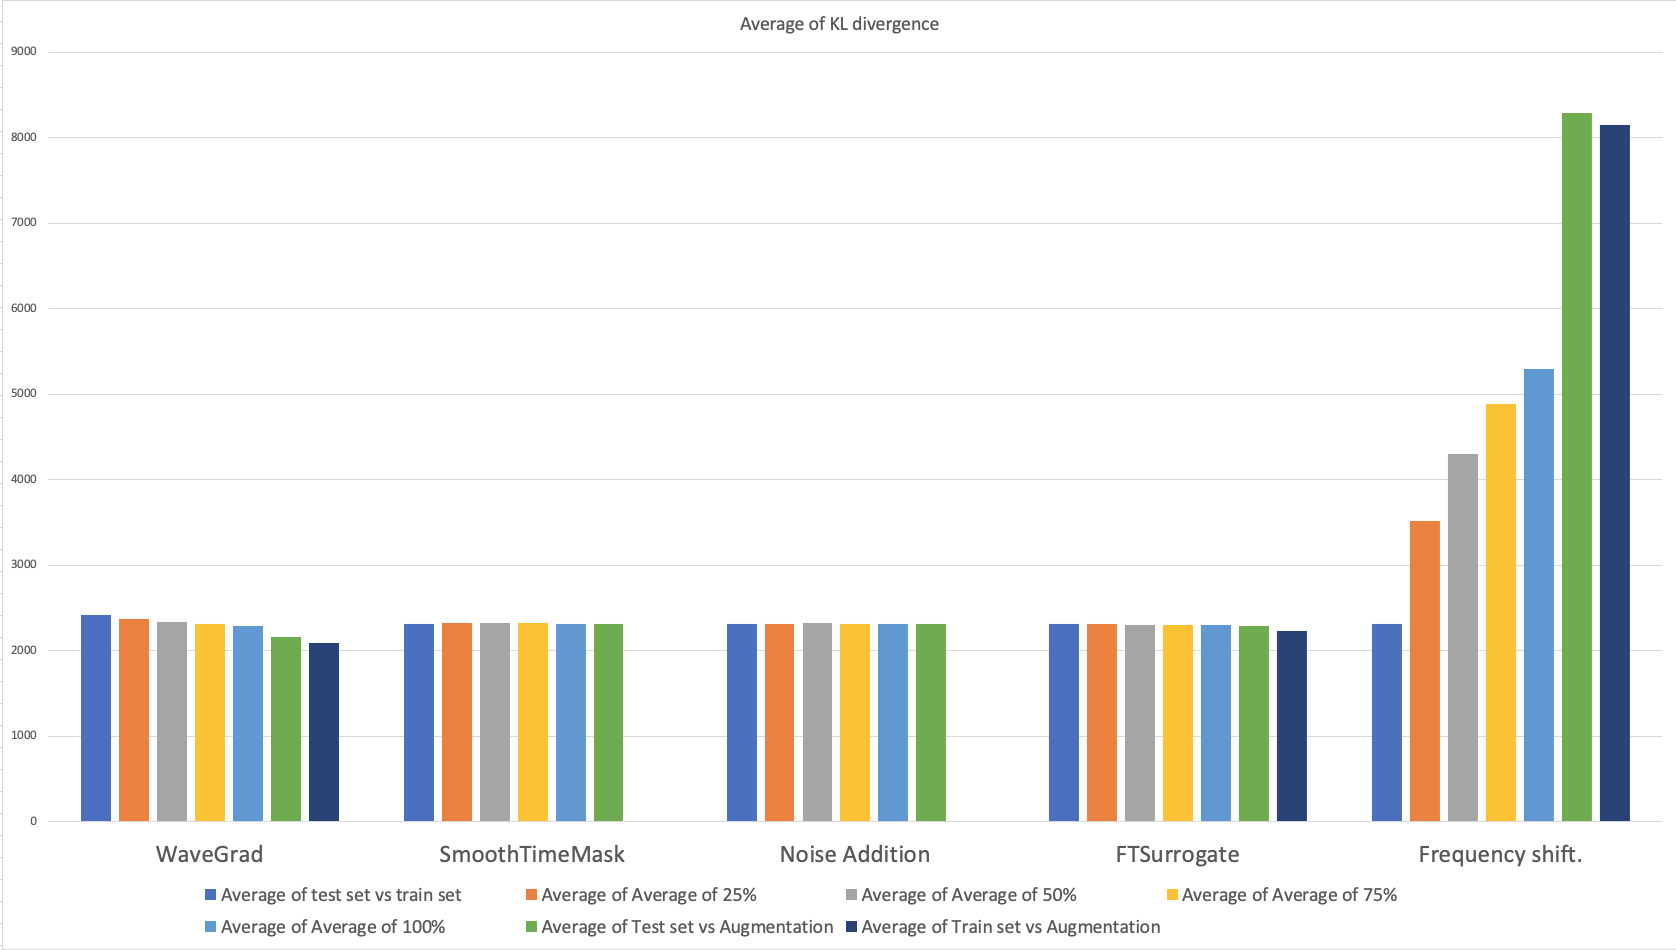
\includegraphics[width=1\textwidth]{fig/Avg_KL.png}
    \label{fig:KL-average}
  \end{figure}

\subsection{Size of augmentation}
We present the impact of data augmentation on the similarity by KL-divergence in Figure~\ref{fig:KL-average}.
This result shows that \texttt{WaveGrad} improves similarity when incurred number of ratio of data augmentation to raw signal.
We present the impact on the accuracy of the ratio of data augmentation to raw signal in Table~\ref{table:AverageAccuracy}.
This result shows that the \texttt{WaveGrad} does not improve the accuracy.

